
\title{Maskinkod}
\section{Maskinkod}


\begin{frame}[fragile,t]
    \begin{block}{\centering\Large Föreläsning 4 --- Maskinkod}

        \halfblankline

        \ti{Förberedelse inför laboration 4}

        \halfblankline
        \begin{itemize}
            \ii{Vad är en dator?}
            \ii{Binära tal}
            \ii{CPU och Minne}
            \ii{Maskinkod och instruktioner}
            \ii{Assembly-språk}
            \ii{Kompilerare och tolkar}
            \ii{\emph{c3pu} -- används på laborationen}
        \end{itemize}

        \halfblankline
    \end{block}

\end{frame}

\begin{frame}[fragile,t]
    \frametitle{Bakgrund}
    \vspace{2em}

    \begin{columns}[T]
        \begin{column}{0.65\textwidth}
            \ti{Varför lära sig Maskinkod?}

            \blankline
            \begin{itemize}
                \ii{Djupare förståelse -- insikt i hur datorer fungerar på en grundläggande nivå.}
                \begin{itemize}
                    \ii{\emph{Vad händer i datorn med kod som vi skrivit?}}
                \end{itemize}
                \ii{Effektiv problemlösning och innovativt tänkande.}
                \begin{itemize}
                    \ii{\emph{Hur kan vi skriva snabb och effektiv kod?}}
                    \ii{\emph{Hur kan vi hitta på innovativa lösningar?}}
                \end{itemize}
            \end{itemize}
        \end{column}
        \begin{column}{0.35\textwidth}
            \vspace{-2em}
            \begin{center}
                \begin{tikzpicture}
                    \only<3->{
                        \node (hl) [rectangle, draw, fill=blue!20, text width=6em, text centered, minimum height=2em] {Högnivåspråk};
                        \node (al) [rectangle, draw, fill=green!20, below=of hl, text width=6em, text centered, minimum height=2em] {Assembly};
                        \node (mc) [rectangle, draw, fill=red!20, below=of al, text width=6em, text centered, minimum height=2em] {Maskinkod};
                        \node (hw) [rectangle, draw, fill=orange!20, below=of mc, text width=6em, text centered, minimum height=2em] {Hårdvara};

                        \draw[->] (hl) -- (al);
                        \draw[->] (al) -- (mc);
                        \draw[->] (mc) -- (hw);
                    }
                \end{tikzpicture}
            \end{center}
        \end{column}
    \end{columns}
\end{frame}


\begin{frame}[fragile,t]
    \frametitle{Vad är en dator?}


    \begin{columns}[T] % The [T] option is used to align the columns content at the top
        \begin{column}{0.6\textwidth}
            \ti{Komponenter}

            \halfblankline
            \begin{itemize}
                \ii{\textbf{CPU:} ALU, kontrollenhet, cache}
                \ii{\textbf{Minne:} RAM och lagring (hårddisk)}
                \ii{\textbf{I/O-enheter:} In- och utmatning (mus, tangentbord, skärm)}
                \ii{\textbf{Moderkort:} Kopplar ihop alla komponenter}
            \end{itemize}

            \blankline
            \ti{Programvara vs. Hårdvara}

            \halfblankline
            \begin{itemize}
                \ii{\textbf{Hårdvara:} Fysiska delarna av datorn}
                \ii{\textbf{Mjukvara (programvara):} Instruktioner för att utföra uppgifter}
            \end{itemize}

        \end{column}
        \begin{column}{0.4\textwidth}
            \begin{center}
                \begin{tikzpicture}[scale=0.8, every node/.style={scale=0.8}]
                    % Define CPU and its internal components
                    \node (cpu) [rectangle, draw, fill=blue!20, minimum height=9.2em, minimum width=9.5em, rounded corners, align=center, label=above:CPU] {};
                    \node (cu) [rectangle, draw, fill=green!30, below=.5em of cpu.north, minimum height=1.5em, minimum width=9em, align=center] {Control Unit};
                    \node (alu) [rectangle, draw, fill=red!30, below=.5em of cu, minimum height=1.5em, minimum width=9em, align=center] {ALU};
                    \node (pm) [rectangle, draw, fill=orange!40, below=.5em of alu, minimum height=1.5em, minimum width=9em, align=center] {Primary Cache};
                    \node (sm) [rectangle, draw, fill=yellow!40, below=.2em of pm, minimum height=1.5em, minimum width=9em, align=center] {Secondary Cache};

                    % Define I/O Devices
                    \node (io) [rectangle, draw, fill=gray!30, below=of cpu, minimum height=3em, minimum width=9.5em, rounded corners, align=center, label=above:I/O Devices] {Mouse, Keyboard,\\Screen, etc.};

                    % Define RAM
                    \node (ram) [rectangle, draw, fill=purple!40, left=of cpu, yshift=-3.1em, xshift=3em, minimum height=15.5em, minimum width=3em, rounded corners, align=center, label=above:RAM] {};

                \end{tikzpicture}
            \end{center}
        \end{column}
    \end{columns}

\end{frame}

\begin{frame}[fragile,t]
    \frametitle{Binära tal - Introduktion}

    \ti{Olika talsystem}

    \begin{itemize}
        \ii{Talsystem används för att representera tal med symboler.}
        \ii{Decimal (bas 10) -- vanligast, använder siffror 0-9.}
        \ii{Siffrors position bestämmer 10-potensvärdet. Exempel:\\
            \halfblankline
            \hspace{5mm}\(274 = 2\cdot 100 + 7\cdot 10 + 4\cdot 1\)\\
            \hspace{5mm}\(274 = 2\cdot 10^2 + 7\cdot 10^1 + 4\cdot 10^0\)}
    \end{itemize}

    \blankline
    \ti{Binärt talsystem}
    \begin{itemize}
        \ii{Binärt (bas 2) -- används av datorer, bara två siffror, 0 och 1.}
        \ii{Varje siffra kallas en \textit{bit}.}
        \ii{Siffrors position bestämmer 2-potensvärdet. Exempel:\\
            \halfblankline
            \hspace{5mm}\(1011_2 = 1\cdot 2^3 + 0\cdot 2^2 + 1\cdot 2^1 + 1\cdot 2^0\)\\
            \hspace{5mm}\(1011_2 = 1\cdot 8 + 0\cdot 4 + 1\cdot 2 + 1\cdot 1 = 11\)}
    \end{itemize}

\end{frame}

\begin{frame}[fragile,t]
    \frametitle{Binära tal - Varför?}

    \ti{Effekten av olika baser}
    \begin{itemize}
        \ii{Basen bestämmer antalet symboler (siffror) som används för att representera tal.}
        \ii{Större bas kräver färre symboler för att representera samma tal.}
        \ii{Exempel:}
        \begin{itemize}
            \is{Talet $999_{10}$ skrivs med 3 siffror}
            \ii{Motsvarande i binärt: $1111100111_2$, 10 siffror.}
        \end{itemize}
    \end{itemize}

    \blankline
    \ti{Varför binära tal i datorer?}

    \halfblankline
    \begin{itemize}
        \ii{Enkelt att representera elektroniskt (ström finns/ström saknas).}
        \ii{Pålitligt att tolka signaler som hög (1) eller låg (0) spänning.}
    \end{itemize}
\end{frame}

\begin{frame}[fragile,t]
    \frametitle{Binära tal - I Datorer}


    \ti{Bits, Bytes och Ord}

    \halfblankline
    \begin{itemize}
        \ii{\textbf{Bit:} Grundläggande enhet av data i datorer (0 eller 1)}
        \ii{\textbf{Byte:} Grupp av 8 bitar}
        \ii{\textbf{Ord:} Processor-specifik grupp av bitar (t.ex., 32-bit eller 64-bit)}
    \end{itemize}

    \blankline
    \ti{Användning av binära tal}

    \halfblankline
    \begin{itemize}
        \ii{Lagring och bearbetning av all data och instruktioner}
        \ii{Varje byte kan t.ex. representera ett litet heltal (0--255) eller ett tecken (ASCII-kod)}
        \ii{Större grupper (ord) hanterar mer komplexa data som heltal och flyttal}
    \end{itemize}

\end{frame}

\begin{frame}[fragile,t]
    \frametitle{Hexadecimala Tal}

    \ti{Hexadecimala talsystemet}

    \begin{itemize}
        \ii{Hexadecimal (bas 16) - använder siffror 0-9 och bokstäverna A-F.}
    \end{itemize}

    \blankline
    \ti{Varför Hexadecimala tal?}

    \begin{itemize}
        \ii{Förenkling!}
        \begin{itemize}
            \ii{Varje tecken representerar fyra binära siffror (bitar).}
            \ii{Lättare att läsa och skriva stora binära tal.}
        \end{itemize}
        \ii{Används ofta för att representera \emph{minnesadresser}}
    \end{itemize}

    \blankline
    \ti{Exempel}

    \begin{itemize}
        \ii{Binärt: \texttt{1011 1010} = Hex: \texttt{BA}}
        \ii{Större binärtal: \texttt{1011 1010 0101 1110} = Hex: \texttt{BA5E}}
    \end{itemize}

\end{frame}




\begin{frame}[fragile,t]
    \frametitle{Central Processing Unit (CPU)}

    \ti{Struktur och funktion}
    \begin{itemize}
        \ii{ALU (Aritmetisk-logisk enhet) -- utför beräkningar och logiska operationer}
        \ii{Register -- lagrar tillfällig data under exekvering}
        \ii{Kontrollenhet -- styr och koordinerar CPU:ns aktiviteter}
        \ii{Cache -- snabbt minne för att optimera åtkomst till data}
    \end{itemize}

    \blankline
    \ti{CPU:n gör:}
    \begin{itemize}
        \ii{Läser instruktioner från minnet}
        \ii{Avkodar (tolkar) dem}
        \ii{Utför instruktionerna (exekverar)}
    \end{itemize}
\end{frame}


\begin{frame}[fragile,t]
    \frametitle{Minne i datorer}

    \ti{Typer av minne}
    \begin{itemize}
        \ii{Hårddisk, SSD, etc. -- permanent lagring av data}
        \ii{RAM -- arbetsminne som lagrar data och instruktioner temporärt}
        \ii{Cache -- snabbare minne nära CPU:n för att optimera åtkomst}
        \ii{ROM -- lagrar permanent data, t.ex. firmware}
    \end{itemize}

    \blankline
    \ti{Var används vilket minne?}
    \begin{itemize}
        \ii{Moderkortet har litet ROM, för att starta datorn}
        \ii{CPU:n kan komma åt RAM via moderkortet}
        \ii{Cache används för att minska åtkomsttiden till ofta använd data\\
            \emph{(Finns ofta flera nivåer av cache)}}
    \end{itemize}
\end{frame}


\begin{frame}[fragile,t]
    \frametitle{Maskinkod -- definition och egenskaper}

    \ti{Vad är maskinkod?}
    \begin{itemize}
        \ii{Binära instruktioner direkt förstådda av CPU:n}
        \ii{Utför enkla operationer som aritmetik, logik, och flyttning av data}
        \ii{CPU:n använder en specifik instruktionsuppsättning (ISA -- \emph{Instruction Set Architecture})}
    \end{itemize}

    \blankline
    \ti{Exempel på maskininstruktioner}
    \begin{itemize}
        \ii{\texttt{MOV}, \texttt{ADD}, \texttt{SUB}, \texttt{JMP}}
    \end{itemize}
\end{frame}

\begin{frame}[fragile,t]
    \frametitle{Maskininstruktioner}

    \ti{Komponenter av en instruktion}
    \begin{itemize}
        \ii{Opcode -- specificerar operationen (t.ex. \texttt{ADD})}
        \ii{Operand(er) -- data eller adresser för operationen (t.ex. register)}
        \ii{Exempel: \texttt{ADD R1, R2, R3}}
    \end{itemize}

    % \begin{envi}
    %     \begin{figure}
    %         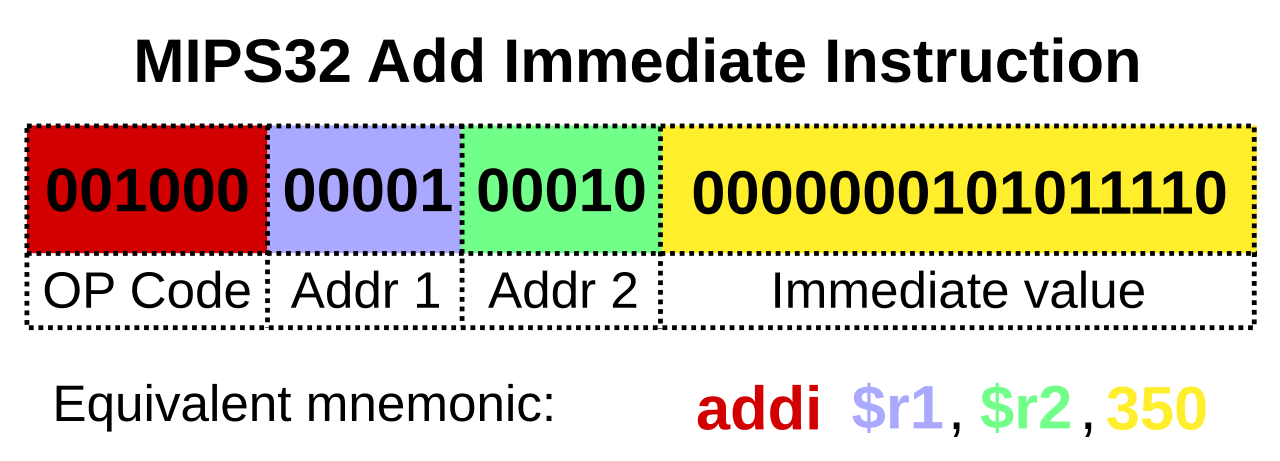
\includegraphics{Mips32_addi}
    %         \caption{By en:User:Booyabazooka - \url{http://en.wikipedia.org/wiki/Image:Mips32_addi.svg}, CC BY-SA 3.0, \url{https://commons.wikimedia.org/w/index.php?curid=1362890}}
    %     \end{figure}
    % \end{envi}

    \blankline
    \ti{Exekvering av instruktioner (fetch-decode-execute)}
    \begin{itemize}
        \ii{CPU:n hämtar instruktionen från minnet}
        \ii{Avkodar opcode och identifierar operand(er)}
        \ii{Utför operationen}
    \end{itemize}
\end{frame}

\begin{frame}[fragile,t]
    \frametitle{Assembly-språk}

    \ti{Vad är Assembly-språk?}
    \begin{itemize}
        \ii{Lågnivåspråk nära maskinkod, använder textrepresentation av instruktioner}
        \ii{Varje assembly-instruktion motsvaras direkt av en maskininstruktion}
        \ii{CPU-specifikt, beroende på arkitektur}
    \end{itemize}

    \blankline
    \ti{Översättning till maskinkod}
    \begin{itemize}
        \ii{Assembler konverterar assembly till maskinkod som CPU:n kan exekvera}
    \end{itemize}
\end{frame}

\begin{frame}[fragile,t]
    \frametitle{Exempel på en assembly-instruktion}

    \ti{Instruktion: \texttt{ADD R1, R2, R2}}
    \begin{itemize}
        \ii{Adderar värdet i \texttt{R1} och \texttt{R2}, lagrar resultatet i \texttt{R2}}
        \ii{R1 och R2 är register som används för temporär datalagring i CPU:n}
    \end{itemize}

    \blankline
    \ti{Relation till maskinkod}
    \begin{itemize}
        \ii{Opcode för \texttt{ADD} + binär representation av register (\texttt{R1}, \texttt{R2})}
        \ii{Exempel: \texttt{ADD R1, R2, R2} $\rightarrow$ \texttt{1001 0001 0010 0010}}
    \end{itemize}
\end{frame}


\begin{frame}[fragile,t]
    \frametitle{Instruktionsuppsättningsarkitektur (ISA)}

    \ti{Vad är ISA?}
    \begin{itemize}
        \ii{ISA specificerar alla maskininstruktioner som en CPU kan förstå och utföra}
        \ii{Olika CPU-arkitekturer har olika uppsättningar}
        \ii{Påverkar hur assembly-språk och maskinkod ser ut för olika processorer}
    \end{itemize}

    \blankline
    \ti{Exempel på ISA:er}
    \begin{itemize}
        \ii{x86 -- Används i de flesta persondatorer}
        \ii{ARM -- Vanlig i mobila enheter}
        \ii{RISC-V -- Öppen arkitektur, växande i popularitet}
    \end{itemize}
\end{frame}

\begin{frame}[fragile,t]
    \frametitle{Maskinkod vs. Högnivåspråk}

    \ti{Utmaningar med maskinkod}
    \begin{itemize}
        \ii{Maskinkod är lågnivå och svår att läsa och skriva för människor}
        \ii{Svårt att hantera tillstånd och strukturer, och att debugga}
        \ii{Inga if/else och loopar -- ersätts med jämförelser och hopp}
        \ii{Funktioner är manuellt hanterade med stack- och registeroperationer}
        \ii{Ingen objektorientering (klasser, arv, etc.)}
    \end{itemize}

    \blankline
    \ti{Varför högnivåspråk?}
    \begin{itemize}
        \ii{Abstraktioner för vanliga strukturer, vilket gör kod enklare att skriva, läsa och underhålla}
        \ii{Kompilatorer hanterar översättning av komplexa strukturer till maskinkod}
    \end{itemize}
\end{frame}


\begin{frame}[fragile]
    \frametitle{Laboration -- \texttt{c3pu}}

        \ti{\large Så, vad ska ni göra på laborationen?}

        \halfblankline
        \begin{itemize}
            \ii{Översätta kod till assembly?}
            \ii{Nej, värre än så \dots}
            \ii{Skriva egen assembly-kod?}
            \ii{Nej, ännu värre än så!}
            \ii{\textbf{Skriva maskinkod för hand!}\\
                \texttt{01010111 01010100 01000110 00100001 00111111}}
        \end{itemize}

\end{frame}

\begin{frame}[fragile]
    \frametitle{\texttt{c3pu} -- Demo}

    \begin{center}
        \Huge DEMO

        {\Large \texttt{c3pu} -- en enkel CPU-simulator}

        \bigskip
        \normalsize\url{https://github.com/lunduniversity/introprog-cpu-emulator/releases/latest}
    \end{center}
\end{frame}